\section{Experiments}
\label{subsec:experiments}

Although the algorithm applied to the PyGame version of Breakout gives
excellent results, the same algorithm applied to the Atari version does not
manage to solve the game correctly, without even satifying the first
temporal goal.
In this section we will analyze the results obtained, also showing some (not all) of the tests that were carried out in an attempt to find out what was the cause of the intractability of Atari's environment. In particular, we will first show the results on PyGame and Atari environments, comparing them. Then we will explain the changes made to the PyGame version during the subsequent test phases. Finally we will draw conclusions from these experiments, analyzing in detail the problems encountered, and we will show some possible changes to be used to address these problems.

\begin{figure}
\centering
\begin{subfigure}[h]{0.3\linewidth}
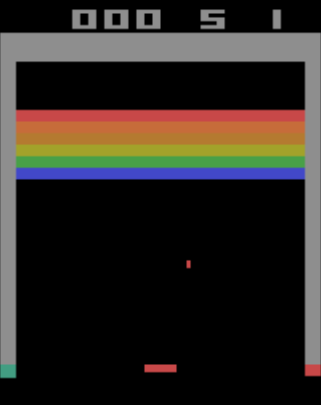
\includegraphics[width=\linewidth]{images/atari-sequence-0.png}
\end{subfigure}
\hfill
\begin{subfigure}[h]{0.3\linewidth}
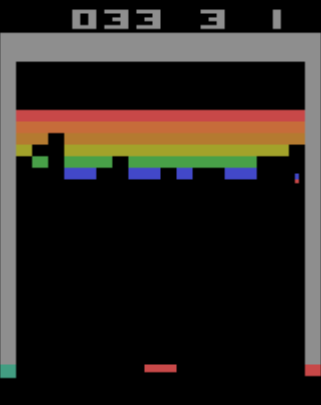
\includegraphics[width=\linewidth]{images/atari-sequence-1.png}
\end{subfigure}
\hfill
\begin{subfigure}[h]{0.3\linewidth}
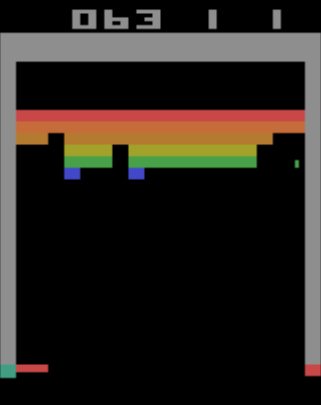
\includegraphics[width=\linewidth]{images/atari-sequence-2.png}
\end{subfigure}
\caption{Sampled frames from the Atari Environment experiments}
\label{fig:atari-sequence}
\end{figure}

\begin{figure}
\centering
\begin{subfigure}[h]{0.8\linewidth}
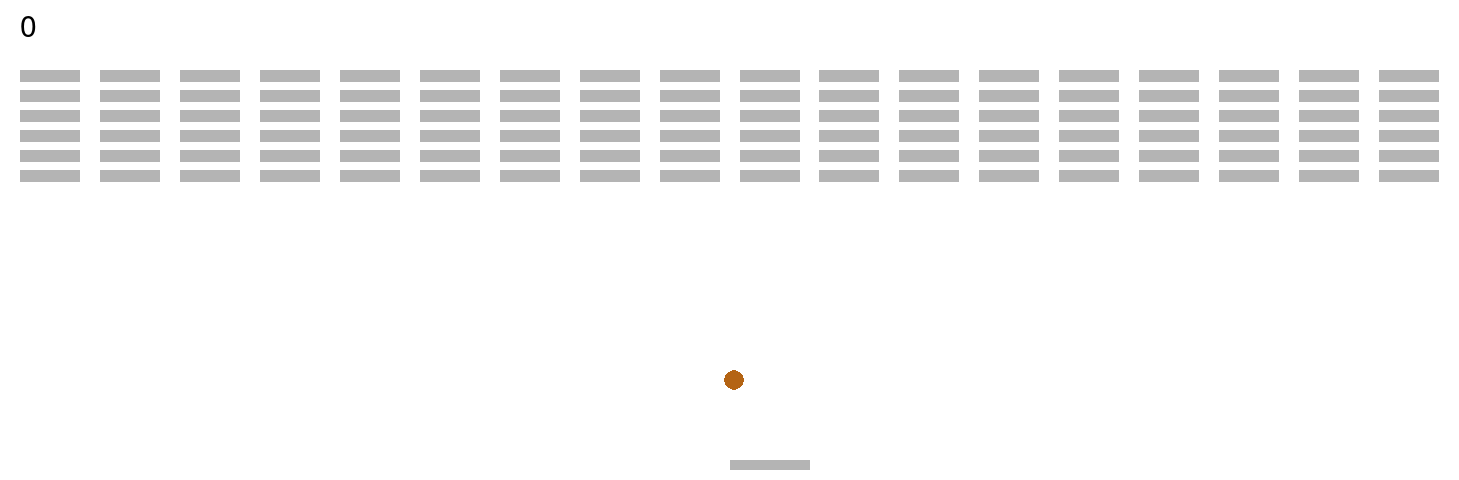
\includegraphics[width=\linewidth]{images/pygame-sequence-0.png}
\centering
\end{subfigure}
\hfill
\begin{subfigure}[h]{0.8\linewidth}
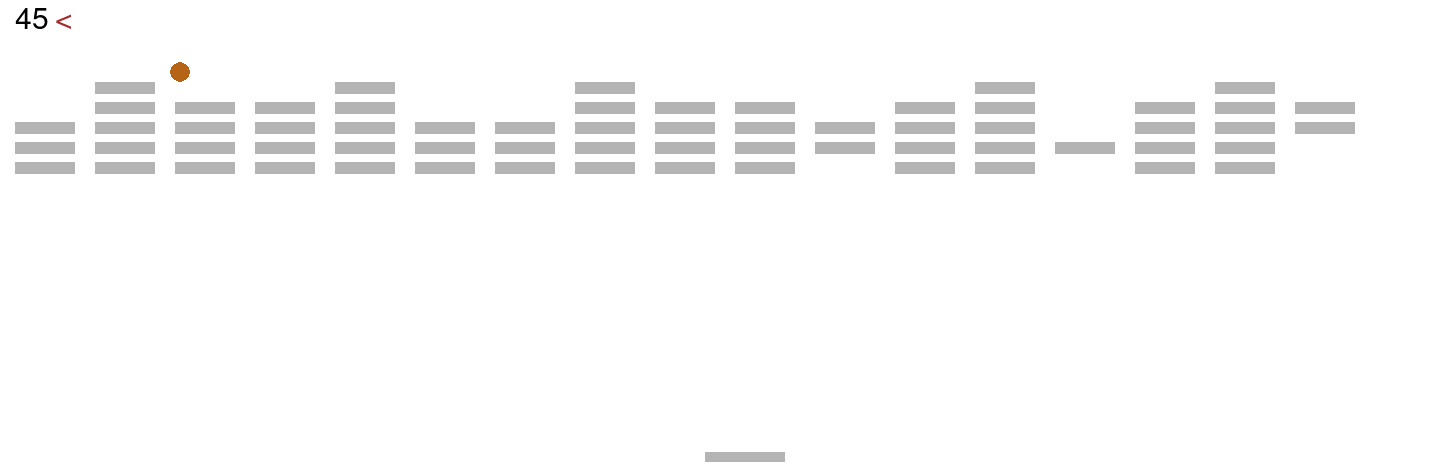
\includegraphics[width=\linewidth]{images/pygame-sequence-1.png}
\centering
\end{subfigure}
\hfill
\begin{subfigure}[h]{0.8\linewidth}
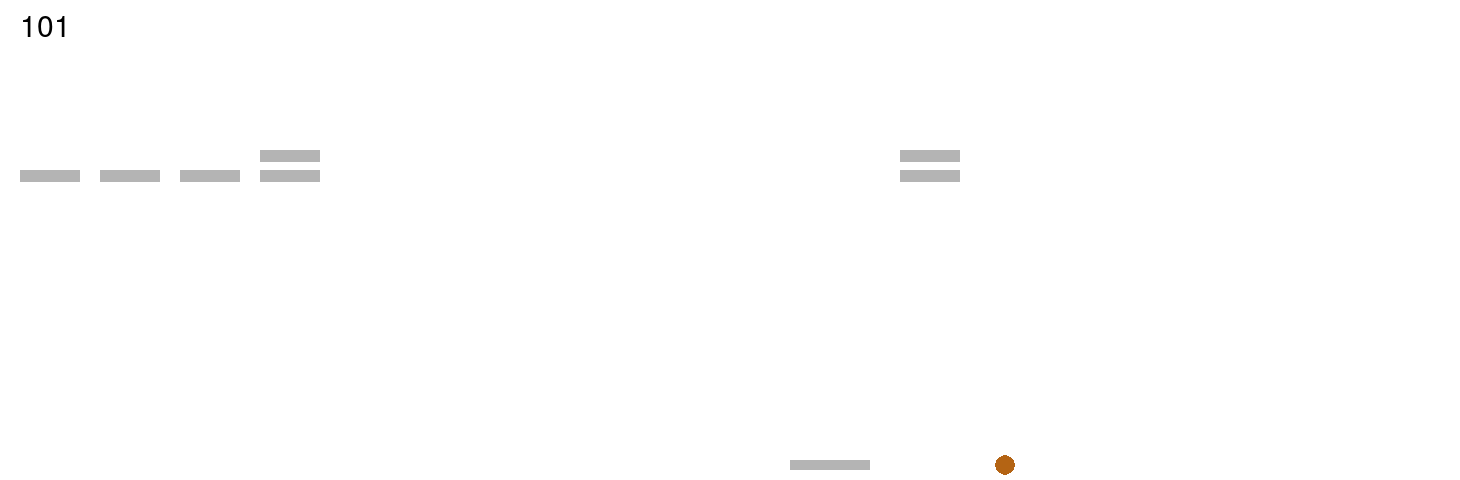
\includegraphics[width=\linewidth]{images/pygame-sequence-2.png}
\centering
\end{subfigure}
\caption{Sampled frames from the PyGame Environment experiments}
\end{figure}

\subsection{PyGame and Atari Results}

The method applied to the environment of PyGame gives excellent results already from 50,000 training periods, while the results obtained by applying the same method to the Atari environment are lower, even after 200,000 epochs. These are the results of the method applied to the two environments:

\begin{table}[h]
	\centering
	\begin{tabular}{*{8}{c}}
		Environment & Epochs & Explored States & Total Reward \\
		\hline
		Atari & 100,000 & 26,291 & 46 \\
		Atari & 200,000 & 26,271 & 63 \\
		\hline
		PyGame & 50,000 & 91,821 & 1010 \\
	\end{tabular}
	\caption{Comparison of the results obtained. All the tests shown in the table were performed with the SARSA algorithm. The tests of the Q-Learning algorithm application did not show significant changes in the final results, therefore they were not shown. It is important to note that the reward is assigned differently in the two environments: PyGame returns a reward of 10 for the destruction of any brick. Atari, on the other hand, returns a reward equal to 1, 4 or 7 for the destruction of a brick, depending on the column in which the brick is located: the bricks higher up give a higher reward.}
\end{table}

\begin{figure}
\centering
\begin{subfigure}[h]{\linewidth}
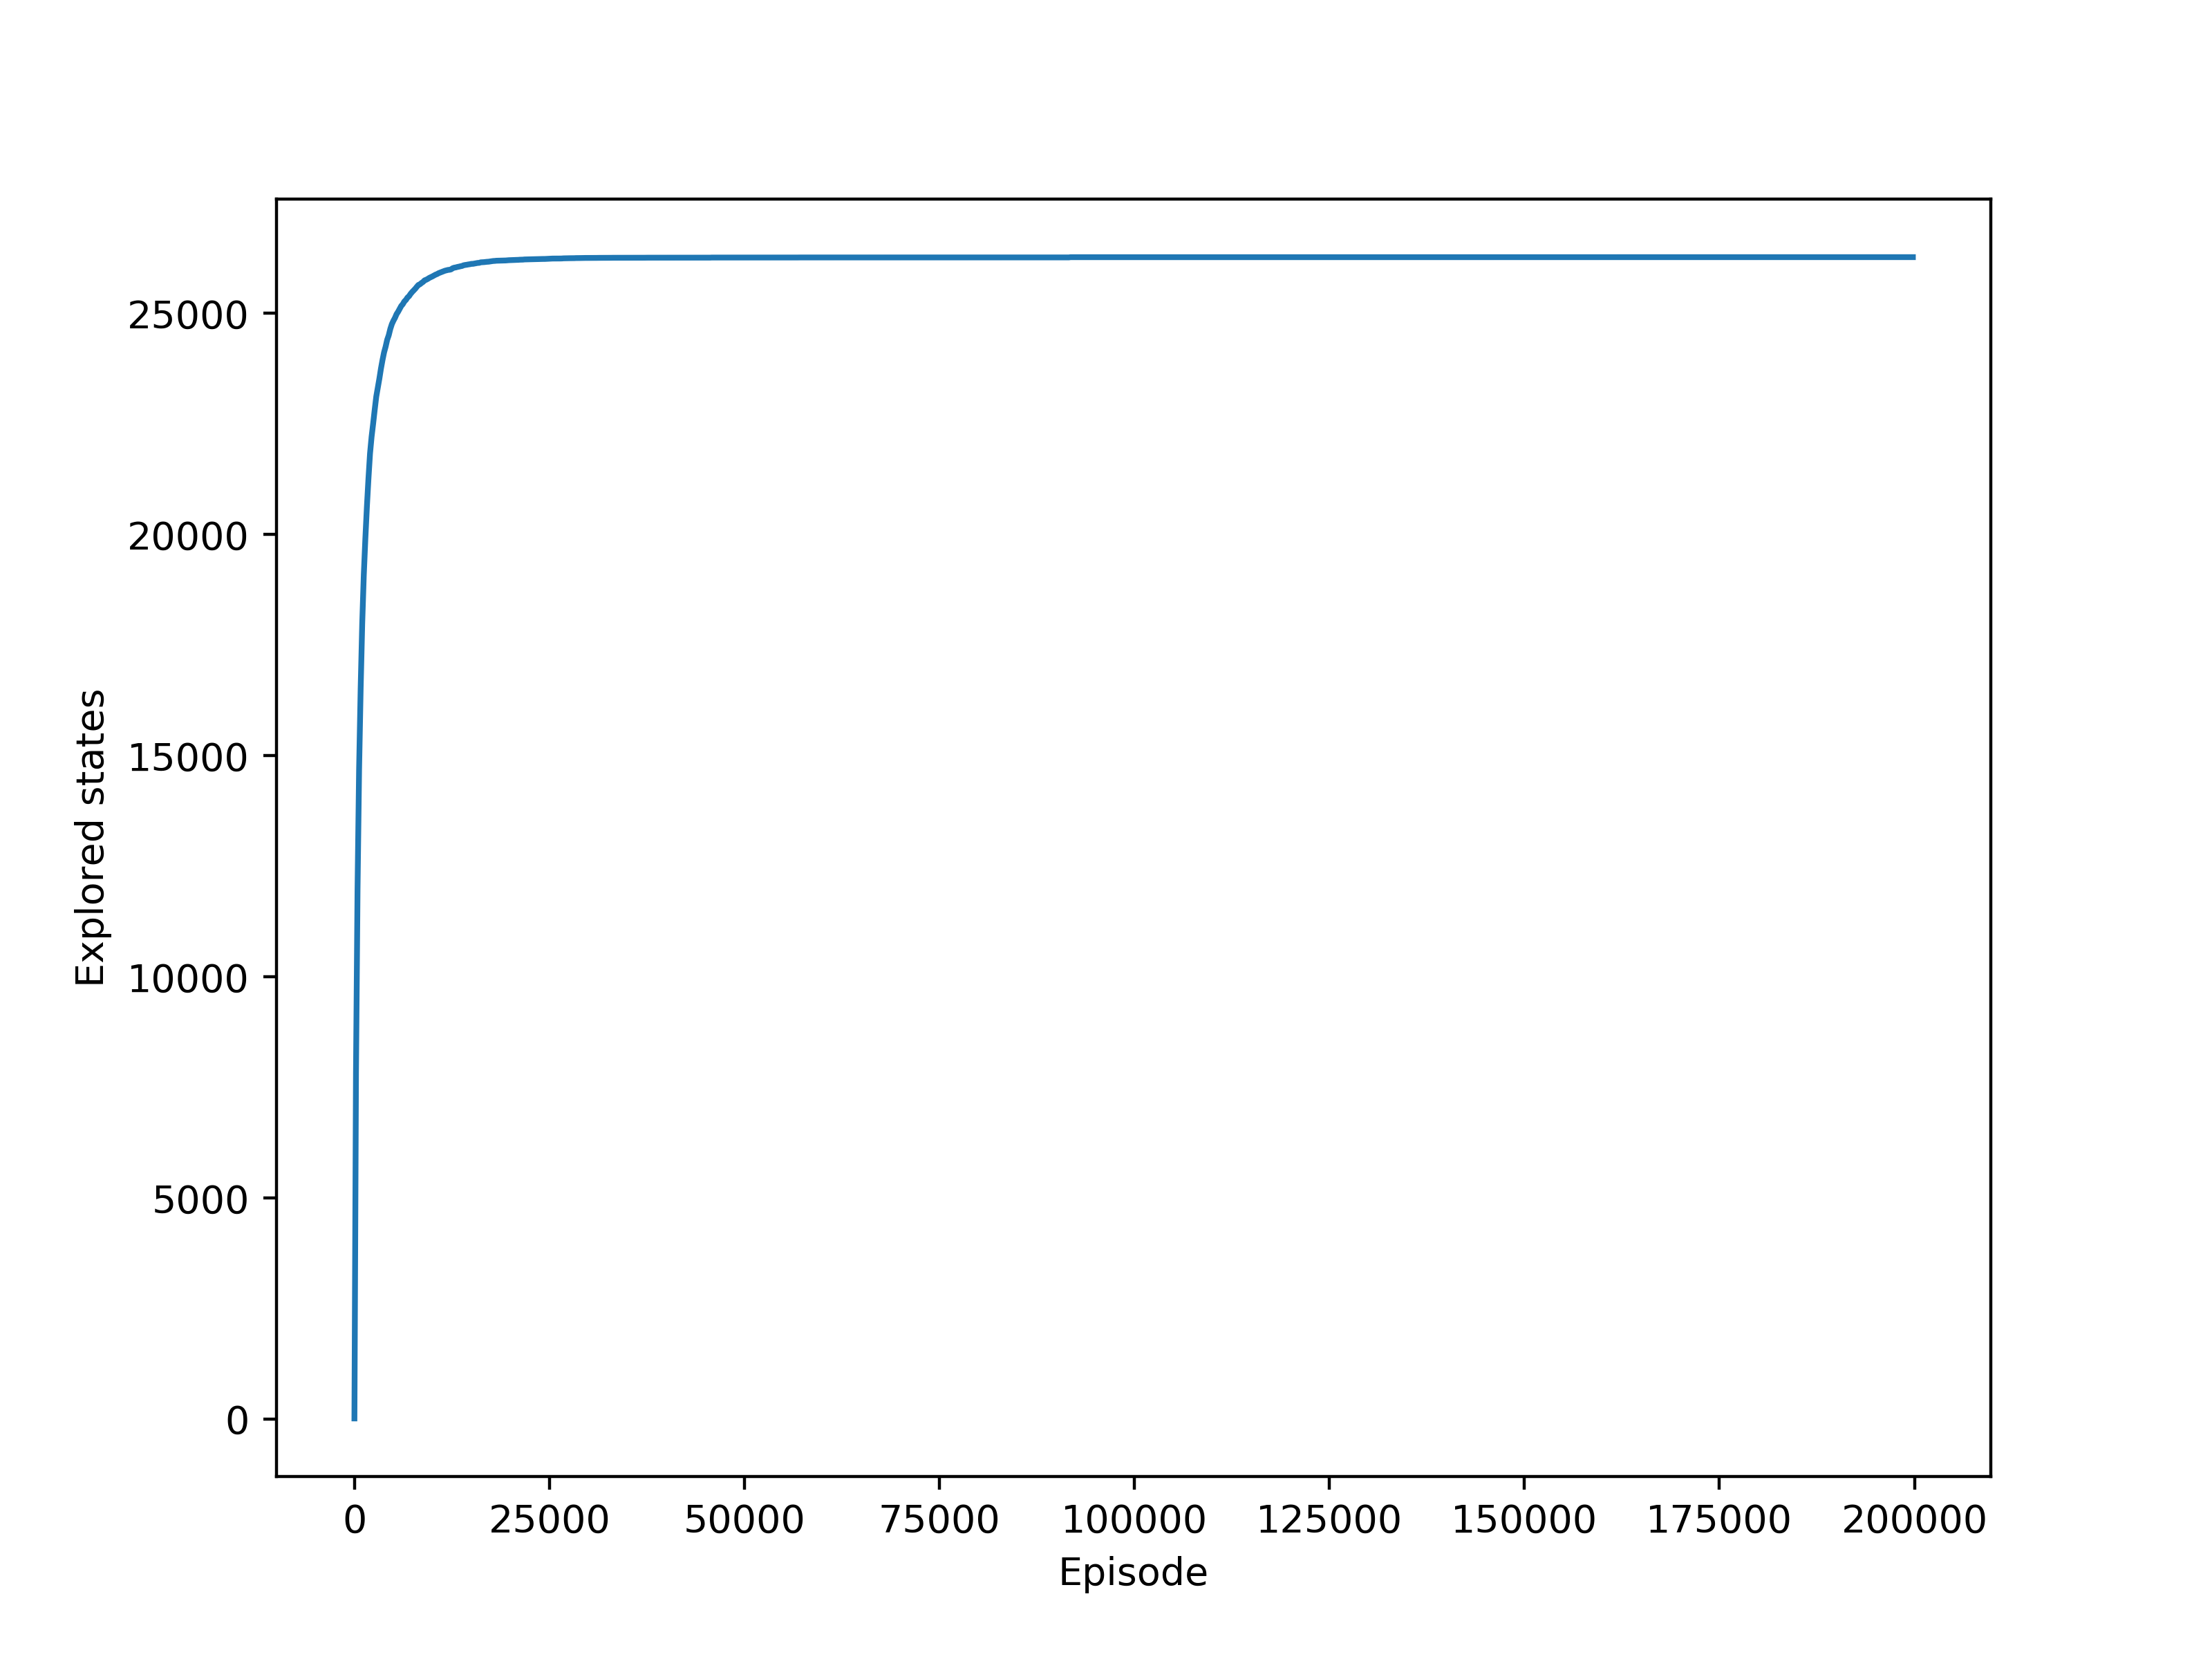
\includegraphics[width=\linewidth]{images/atari-sarsa-explored-states.png}
\centering
\end{subfigure}
\hfill
\begin{subfigure}[h]{\linewidth}
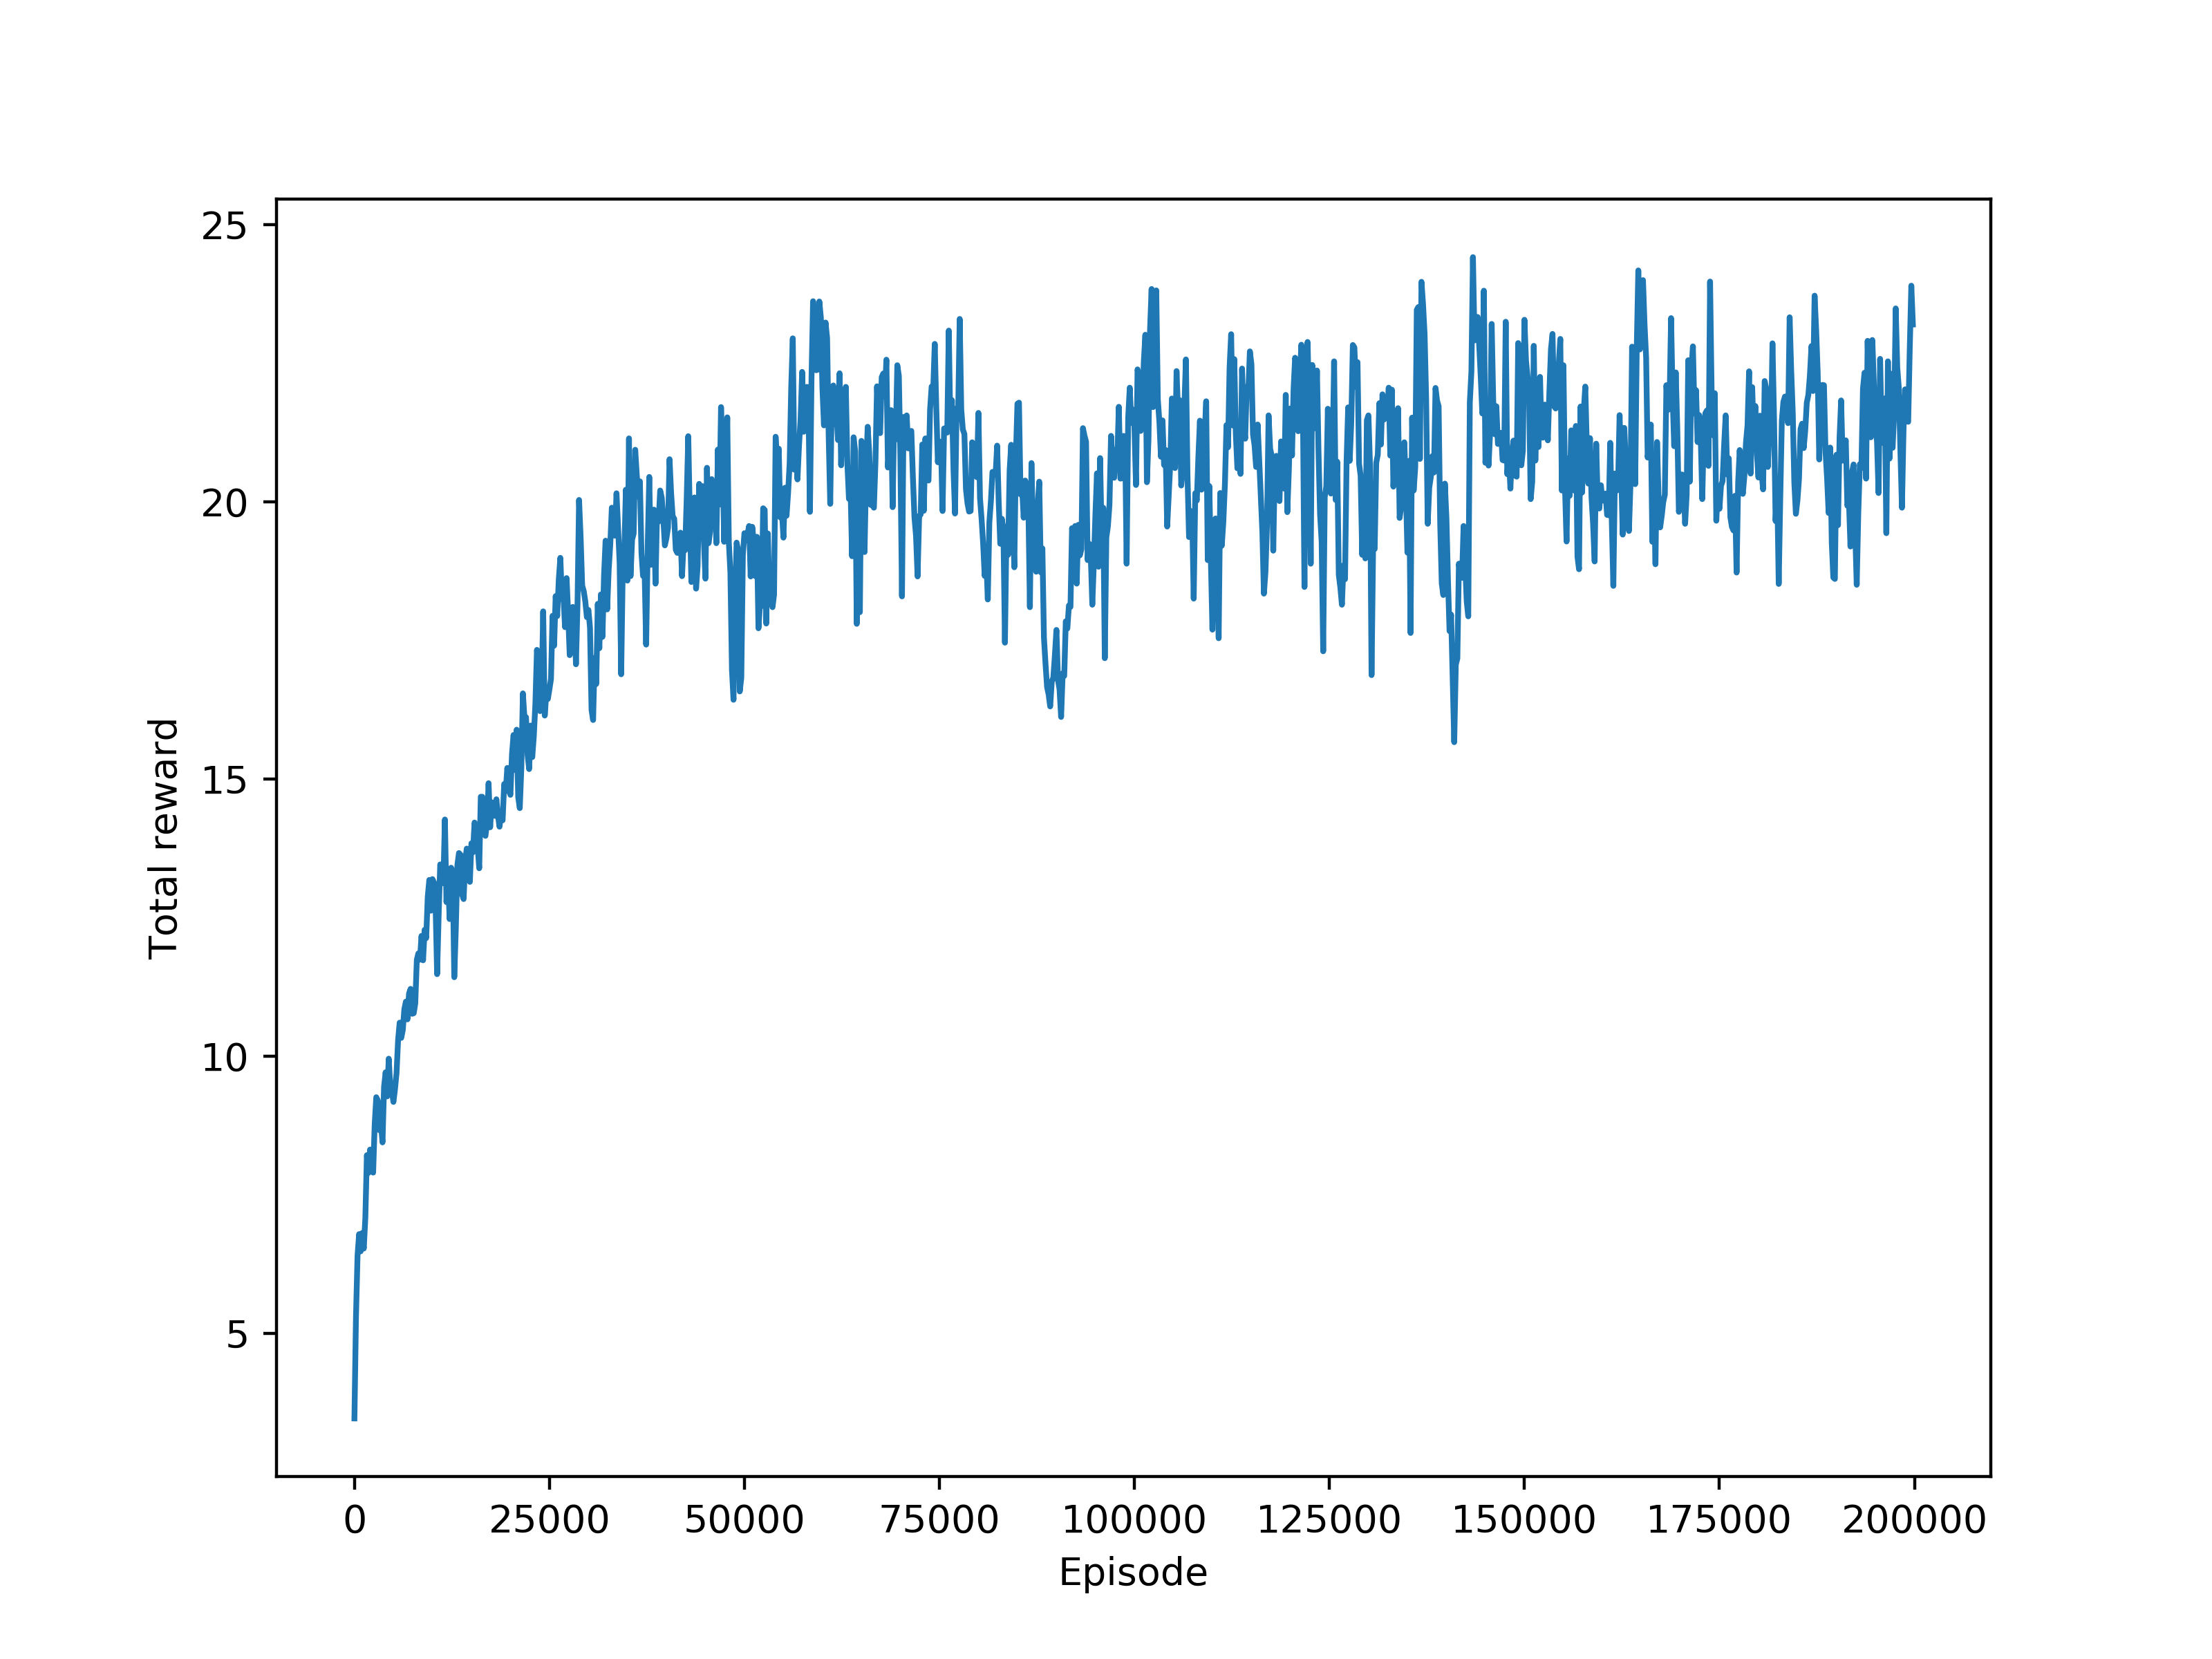
\includegraphics[width=\linewidth]{images/atari-sarsa-total-reward.png}
\centering
\end{subfigure}
\caption{Plots from the Atari Environment experiments. The reinforcement learning algorithm used in this experiment is SARSA.}
\end{figure}

\begin{figure}
\centering
\begin{subfigure}[h]{\linewidth}
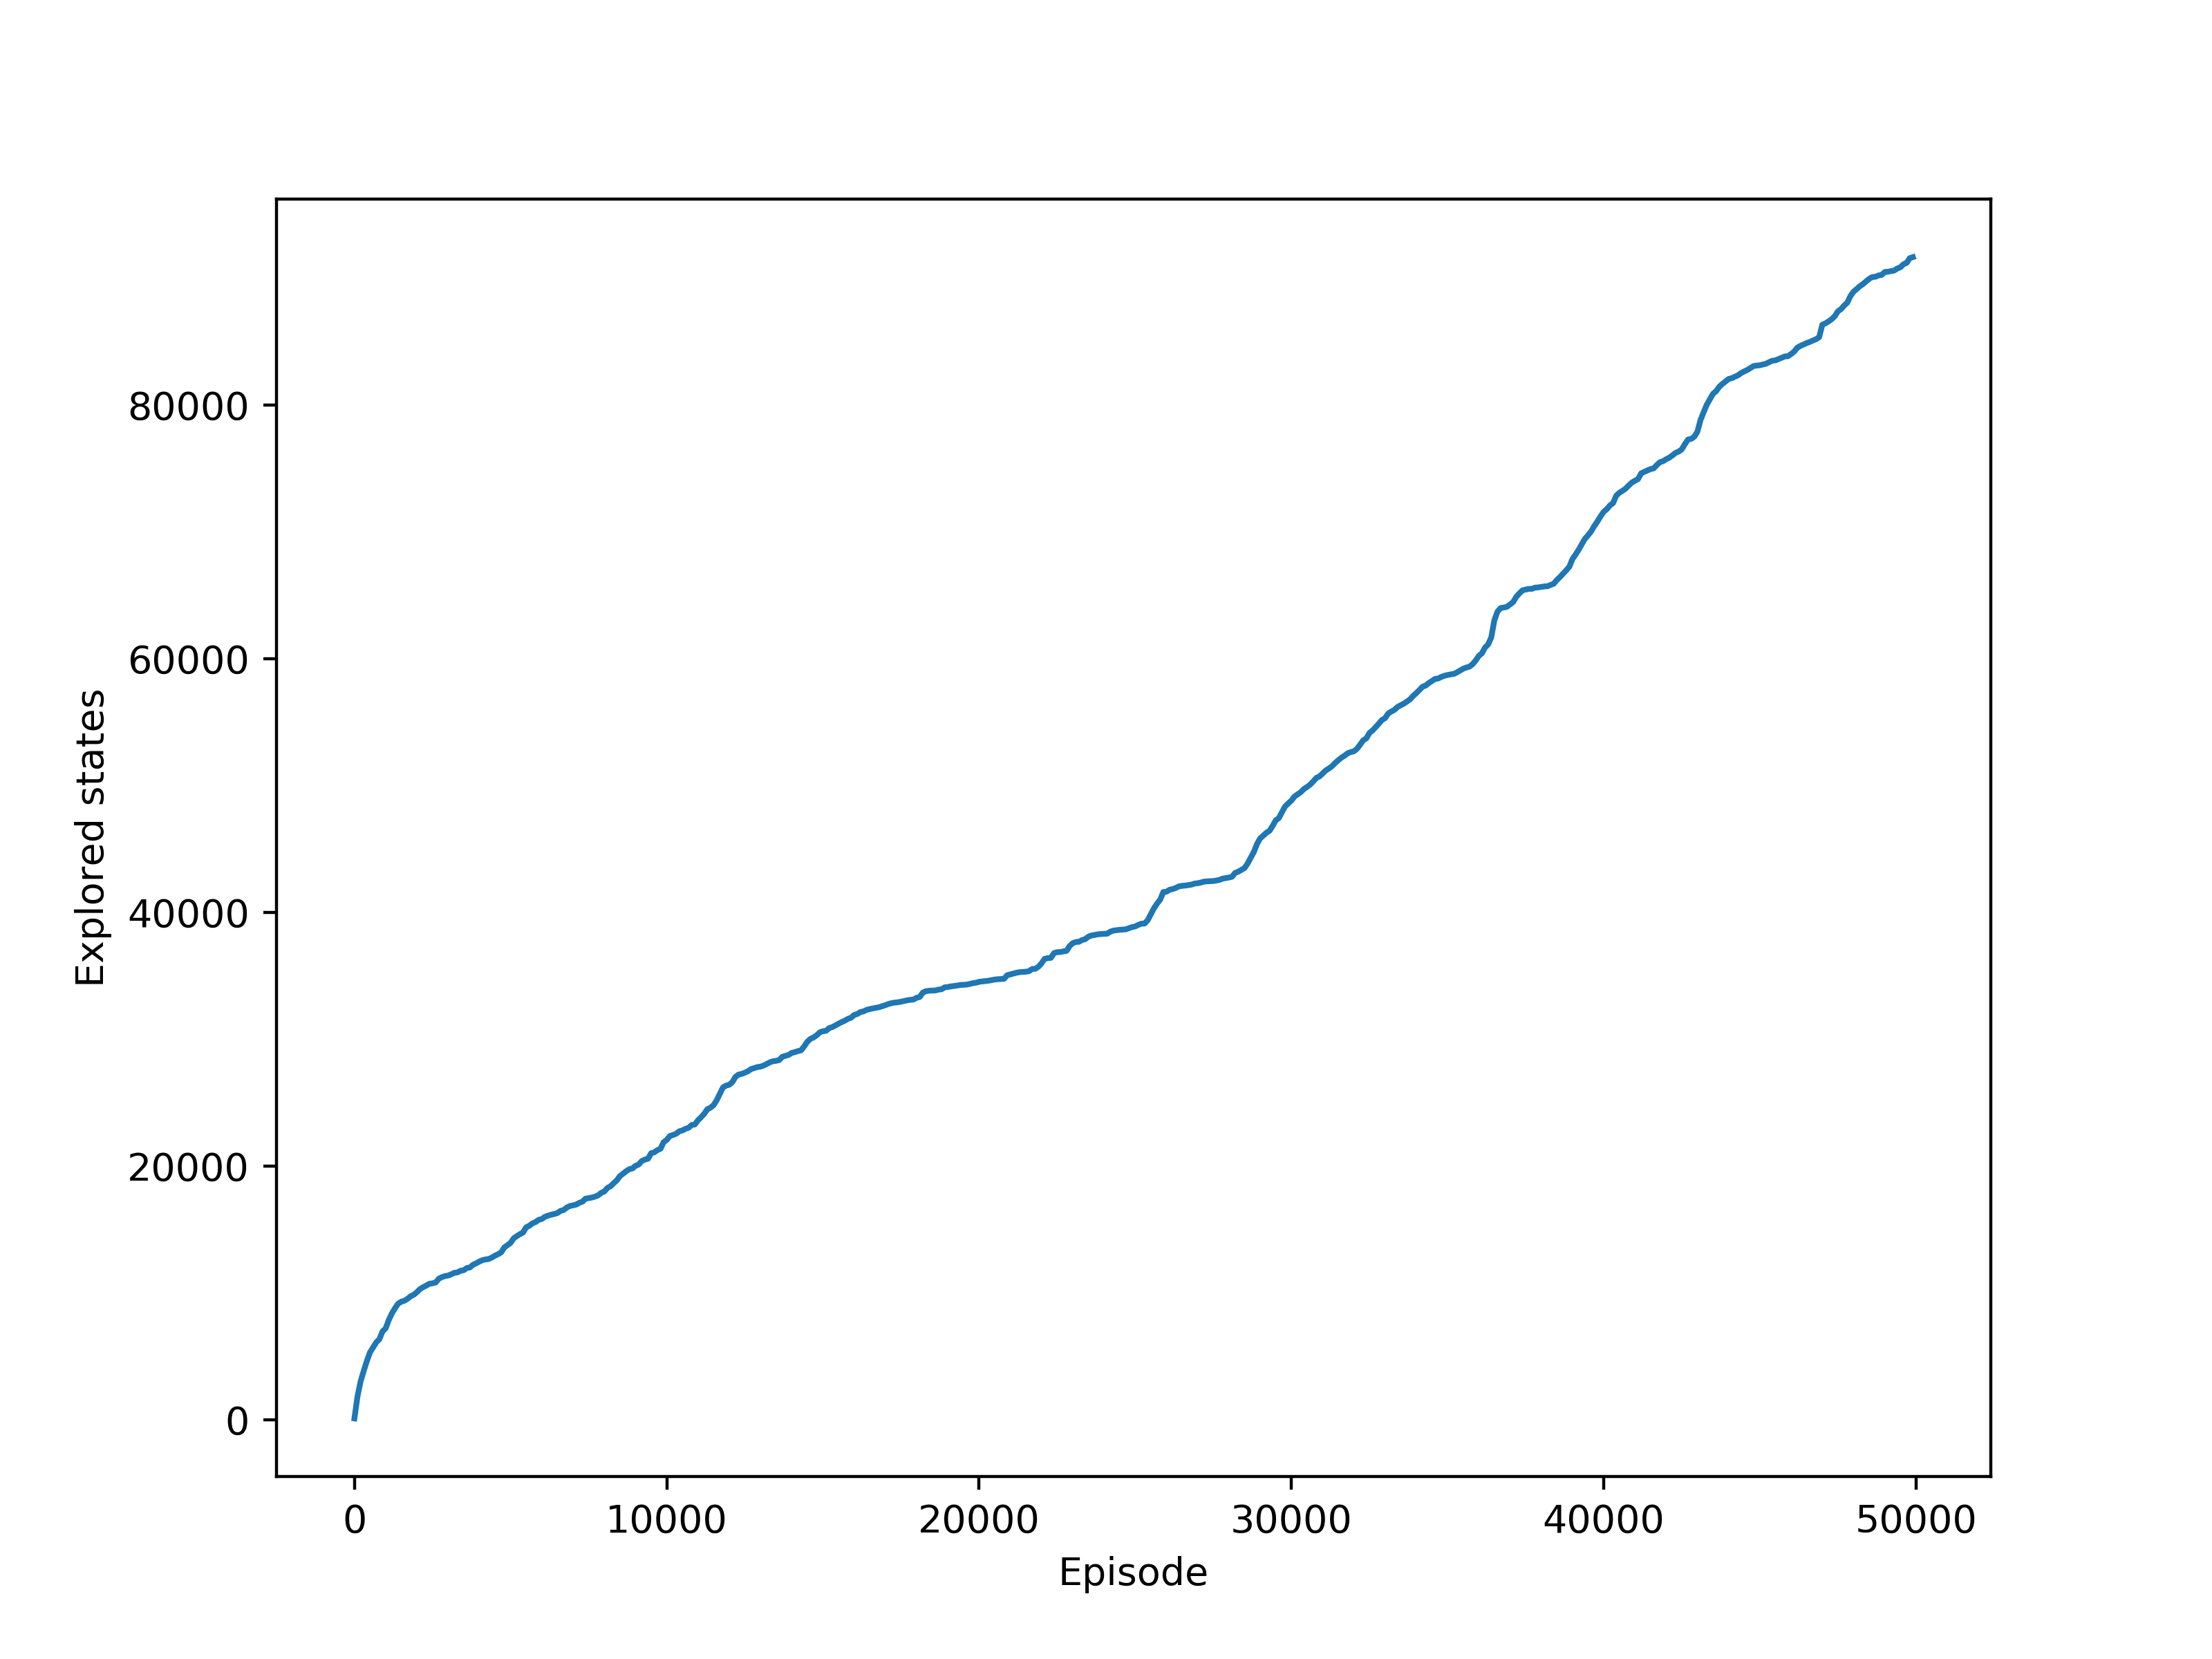
\includegraphics[width=\linewidth]{images/pygame-explored-states.png}
\centering
\end{subfigure}
\hfill
\begin{subfigure}[h]{\linewidth}
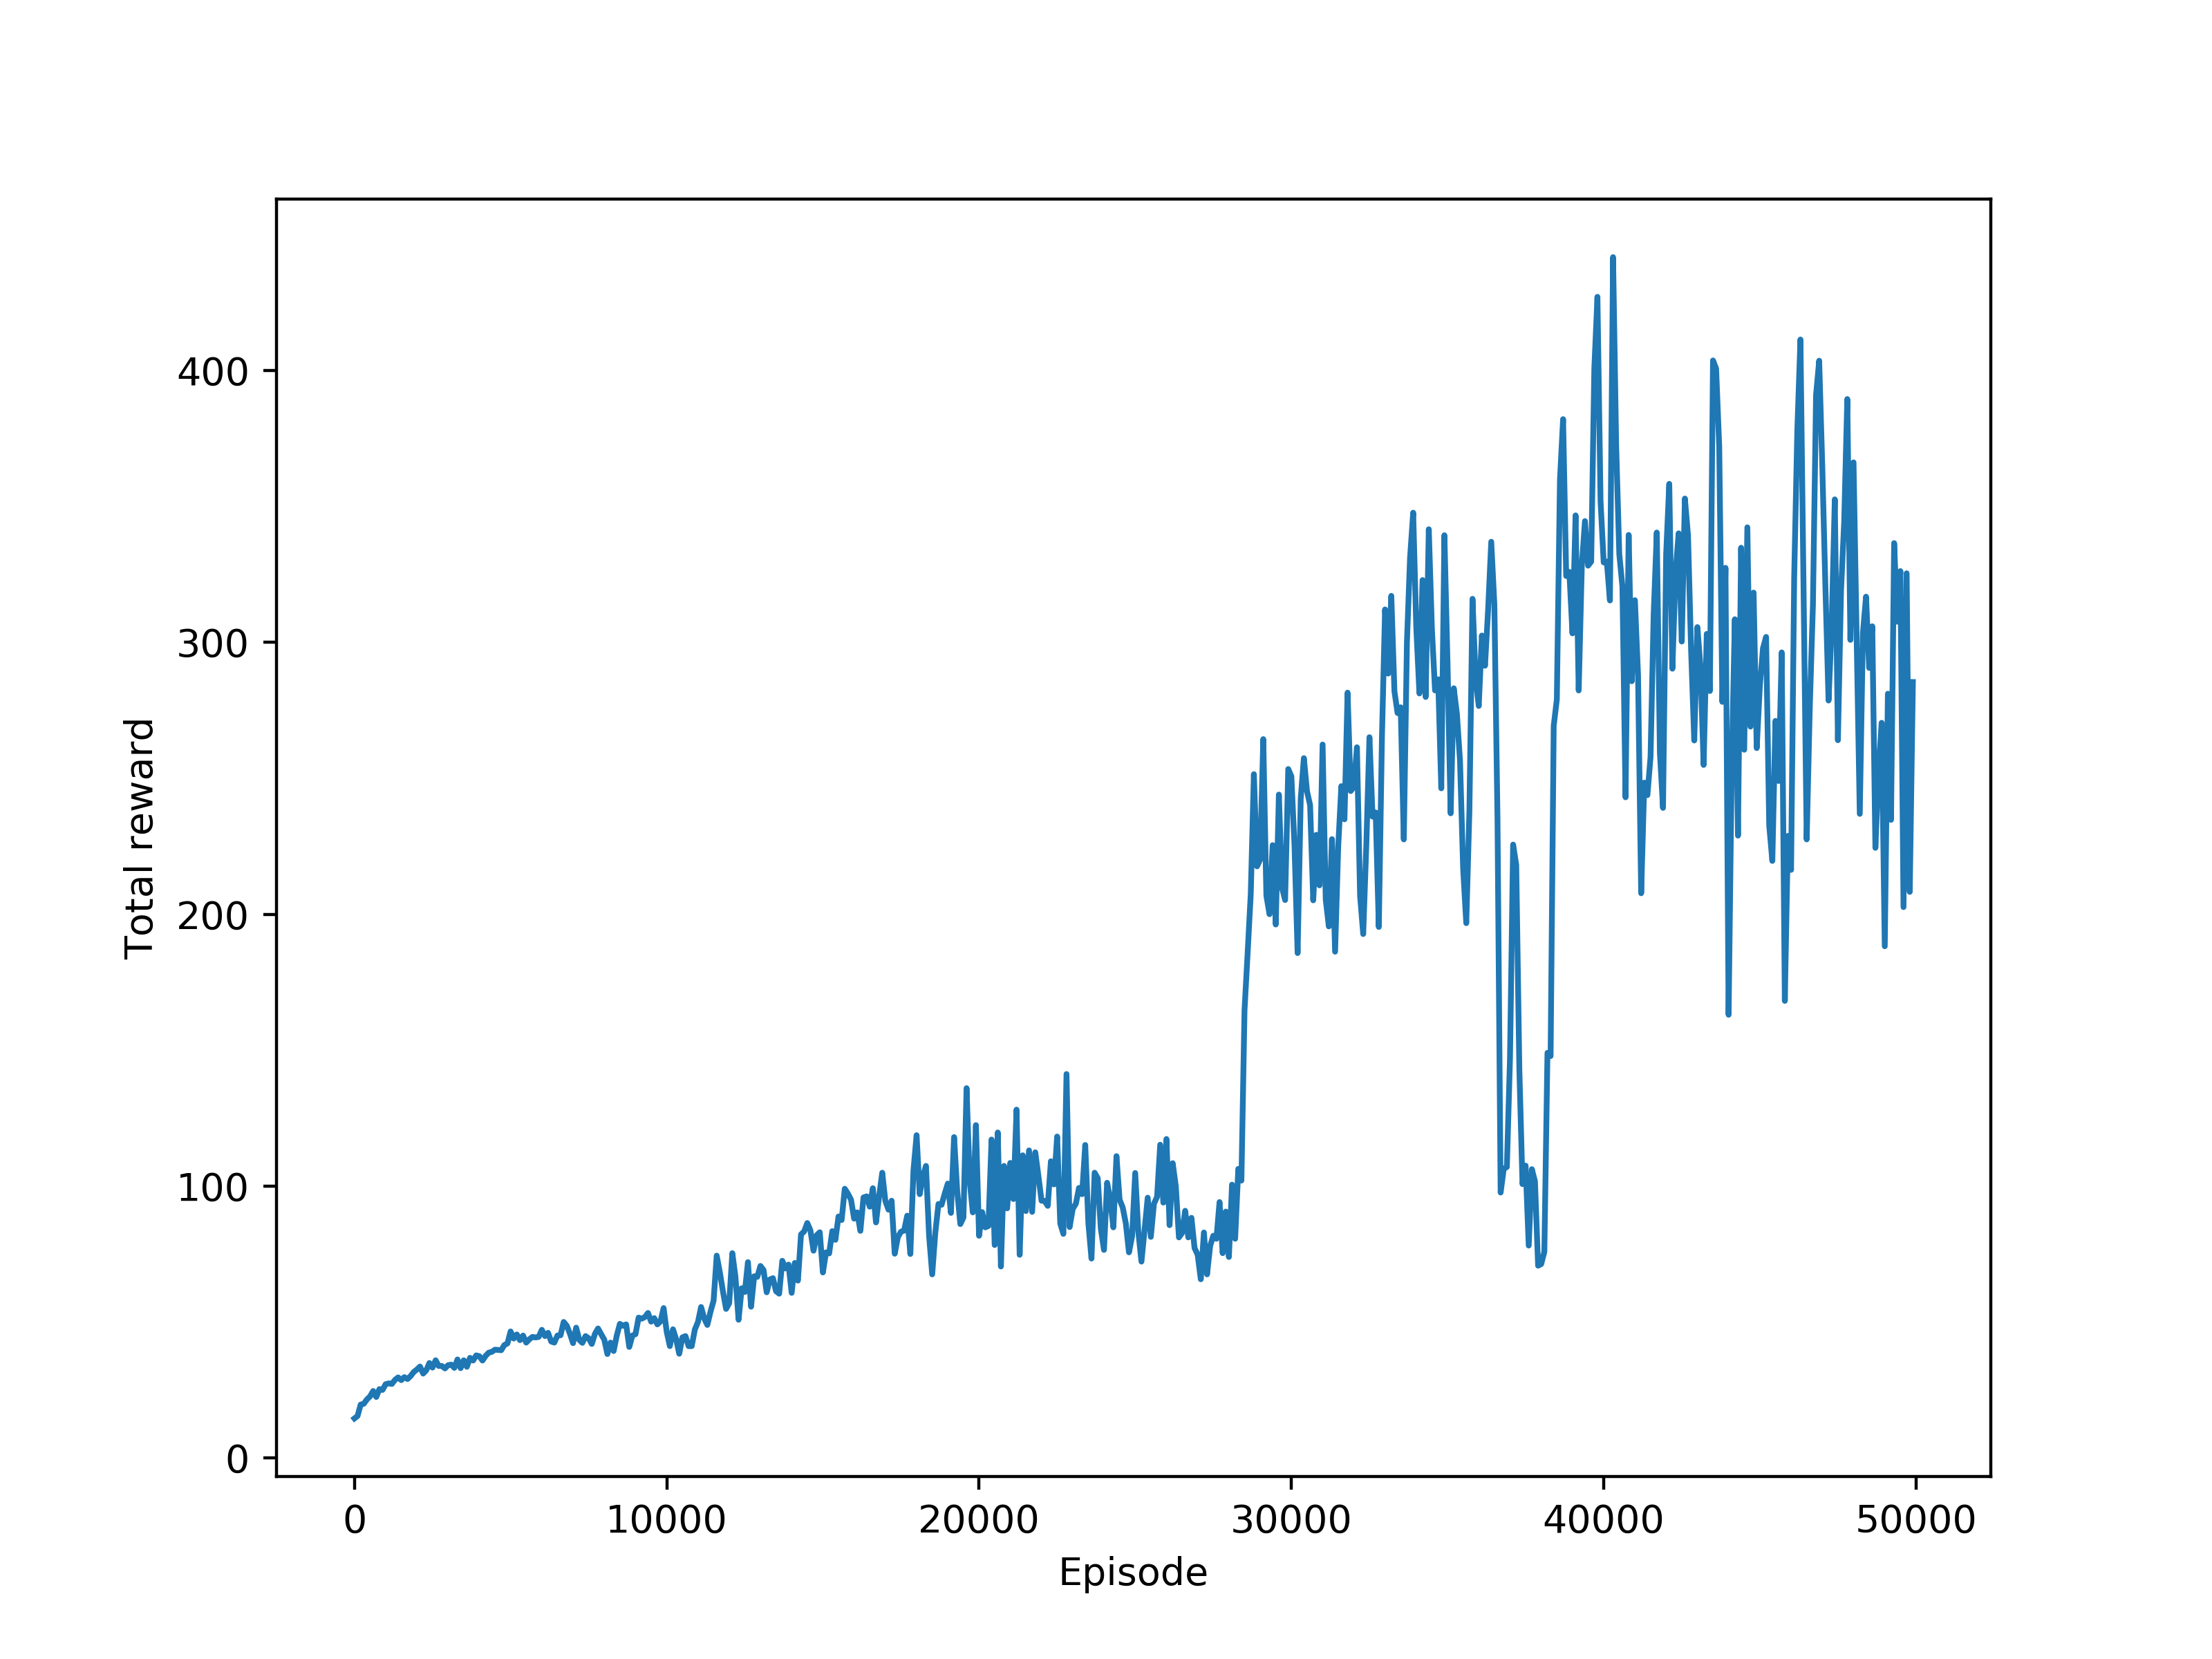
\includegraphics[width=\linewidth]{images/pygame-total-reward.png}
\centering
\end{subfigure}
\caption{Plots from the PyGame Environment experiments. The reinforcement learning algorithm used in this experiment is SARSA.}
\end{figure}

As you can see, the results are much lower in the second case. In an attempt to improve the Atari results, changes in the code have been tested: we have reduced the size of the state space, either the ball space or the paddle space, or its movement space; we have tried to completely remove the information concerning the movement of the paddle; we tested a one-shot version of Atari, in order to make it similar to PyGame and finally we have tried combinations of the above ones. These are the results of these tests:

\begin{table}[h]
	\centering
	\begin{tabular}{*{8}{c}}
		Ball X & Ball Y & Angle & Paddle & Move & Lives Count & Frame Skip & Score \\
		\hline
		144 & 157 & 10 & 144 & 49 & 1 & 4 & 6 \\
		144 & 157 & 10 & 144 & 49 & 5 & 4 & 4-20 \\
		8 & 18 & 10 & 8 & 49 & 1 & 4 & 5 \\
		144 & 157 & 10 & 144 & 10 & 1 & 4 & 7 \\
		144 & 157 & 10 & 144 & 0 & 1 & 4 & 7 \\
		144 & 157 & 10 & 144 & 0 & 5 & 4 & 2-16 \\
		8 & 18 & 10 & 8 & 10 & 1 & 4 & 6 \\
		8 & 18 & 10 & 8 & 0 & 1 & 4 & 2 \\
		8 & 18 & 10 & 8 & 0 & 5 & 4 & 5-15 \\
		\hline
		144 & 157 & 10 & 144 & 13 & 5 & 14 & 19 \\
		144 & 157 & 10 & 144 & 13 & 5 & 10 & 24 \\
		144 & 157 & 10 & 144 & 13$^1$ & 5 & 10 & 16 \\
		144 & 157 & 10 & 144 & 121 & 5 & 10 & 24 \\
	\end{tabular}
	\caption{The first five columns indicate the state space of the related variables, the sixth column indicates the number of lives per game, the sequential column indicates the number of game-frames for each state-frame (see point 6.3.2). The last column indicates the score at the end of the game, expressed as the number of bricks destroyed. In some cases (only those with more than one life) we have specified both the score at the end of the first life and the score at the end of the last life, separated by a dash. All tests were performed with 5000 training epochs. The results of these tests indicate that the score improves with the increase of the lives and the frame skip, with an optimal number of frame skip equal to 10 (not all the tests we performed have been included in this table), while the size of the state space has little influence on the score obtained. $^1$ This test was performed with the same hyperparameters as the previous test, but with a different calculation of the move variable: instead of distributing the 13 states of the move variable from -60 to +60 motion pixels, they were distributed over the range [-40 , +40], cropping excess values.}
\end{table}

Given the number of tests to be performed, we performed them with a low number of training periods, 5000, for obvious reasons of time. So it is necessary to take this data with a grain of salt. But it is still possible to see a trend: the reduction of the state space does not significantly improve the result you get, while giving Atari environment the opportunity to play all his 5 lives worsens the score obtained at the end of the first life, but increases the total score. This is a consequence of the fact that there are no penalties in the reward associated with losing a life: there are only positive rewards given by the destruction of a brick or the achievement of a temporal goal. This makes possible scenarios in which, after losing a life, the paddle succeeds in destroying a brick in the next life, which leads to a reward for the sequence of state-action pairs that led to that result. All this makes the training of AI very random, because the life in which it will take the reward is random, with the risk of losing lives uselessly. We will draw further conclusions later in this section.

\subsection{Modified PyGame}

In the previous point we tried to identify strategies for managing the state space and lives to improve the score, but despite this the difference between the two environments is still large. It is true that PyGame Breakout has a very small state space, but nevertheless decreasing the state space in Atari Breakout to make it similar to PyGame does not produce any improvements. So instead of making Atari similar to PyGame, let's try to do the opposite. There are indeed considerable structural differences between the two environments: the size of paddle, ball, bricks, window and placements of objects in the field. Moreover, the movement of the ball is much slower in PyGame than in Atari: the ball, to reach the first bricks from the paddle, takes 35 frames in PyGame, and only 15 in Atari. In 1500 frames of PyGame it can only destroy 10 bricks, in 1500 frames of Atari it destroys 29 bricks, even 47 with 2000 frames! Remind that a frame corresponds to a state in which you choose an action to move to the next state. In order to better compare the two environments, in an attempt to understand the problems inherent to Atari, we gradually approximated PyGame to Atari, to make the two environments identical.

\begin{figure}
    \centering
    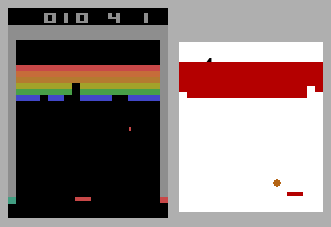
\includegraphics[width=0.7\textwidth]{images/modified-pygame-comparison.png}
    \caption{Comparison between the Atari environment and the modified version of the PyGame environment}
\end{figure}

To do this we changed the PyGame code at some points. In doing so it was highlighted a bug that was already present in PyGame, but that did not show up in its original version:

\lstinputlisting[caption=A more sophisticated version of the ball rebound algorithm.,
    language=Python]{implementation/Breakout-hit-detection-function.py}

We quickly solved it and compared the two environments that we obtained. Despite all these efforts, the difference between the results obtained by applying the method on one environment rather than another is still large: the modified PyGame still manages to produce good results, event with just 5000 epochs of training. It has been noted, however, that PyGame uses an internal reduction of the actually used states: when the ball is lower in the screen, the ball and paddle positions are calculated with greater resolution. We tried to use this resolution reduction algorithm in Atari, but the results were once again disappointing. We even found a worsening effect of the score.

\lstinputlisting[caption=The resolution reduction algorithm inside the get state function.,
    language=Python]{implementation/Breakout-get-state-function.py}

After all these futile attempts we have finally managed to identify the problems of Atari, which are summarized in the next point.

\subsection{The Atari Breakout Difficulties}

In this point we will analyze the intrinsic problems in Atari that prevent the achievement of good results with the method used. One has already been addressed in point 1, which concerned the use of an environment with more lives. Here we will describe the problems of the state space, of the local maximum, of non-determinism and of the collision of states.

\subsubsection{The Dimension Space Problem}

The problem of the size of the state space was clear from the beginning. Before testing it, PyGame had only been used with a 3x3 brick matrix. Atari, on the other hand, has a fixed-size matrix equal to 6x18, which makes both the automaton defining the temporal goals and the size of the playing field larger, in proportion to the paddle size. As explained up to here, there have been many attempts at reducing the state space in Atari, to the extent that it made that dimension identical to that of PyGame, and all attempts proved to be unsuccessful. They did not produce significant improvements in the score, and sometimes even showed a worsening. In fact, it is possible to notice from the number of states visited at each epoch that the speed with which the AI explores new states falls after some threshold, despite maintaining a low score. The algorithm therefore has difficulty in exploring new states, which can have two explanations: there are too many states, and the algorithm get lost, or the problem is not about the number of states, is about the inability of the algorithm to learn, probably due to a collision of states (see below).

\subsubsection{The Local Maximum Problem}

The artificial intelligence algorithm that must learn to maximize the reward
must face a problem of local maximum. In fact, there are many states from
which it is difficult to escape. Take the case in which the paddle hits the
ball in the lower left corner. If the ball tends to go to the right as a result
of the action, there is the possibility that it will fall back into the
opposite corner, lower right. If this is the case, the paddle will have to move
multiple times, before it can get a new reward. In particular, we need a series
of subsequent ``go right'' actions, which make it possible to continue the game.
This is very unlikely, because, in the presence of new states, the choice of
action to be taken is random. And there's a second problem: the difficulty
introduced by a greater number of possible actions: while on PyGame there are
only three actions (``go left'', ``go right'', ``stay still''), on Atari there is a
fourth possible action, which is needed to spawn the ball at the start of the
game, or when a life is lost. This action is automatically performed by the
environment on the aforementioned occasions, but it has not been possible to
prevent the execution of these actions during the normal course of the game.
So the correct action to be taken (``go right'') must be chosen randomly by a
group of 4 actions (25\% probability of choosing the correct action) instead
of 3 (33\%). And if, say, the number of times to perform the ``go right'' action
is N, the probability of this happening is $25\%^N$, which falls below
1\% already for N = 4. If we analyze the moments in which the paddle drops the
ball in the training carried out, we note that most of them are just the cases
described here, in which the paddle is in a corner of the screen and does not
move, sign that no rewards have been discovered for any action, and the ball
falls in the opposite corner.

\begin{figure}
\begin{subfigure}[h]{0.19\linewidth}
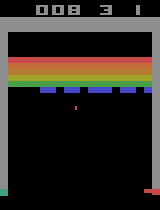
\includegraphics[width=\linewidth]{images/frame-sequence-0.png}
\end{subfigure}
\hfill
\begin{subfigure}[h]{0.19\linewidth}
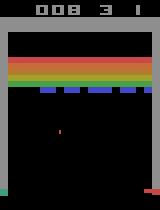
\includegraphics[width=\linewidth]{images/frame-sequence-1.png}
\end{subfigure}
\hfill
\begin{subfigure}[h]{0.19\linewidth}
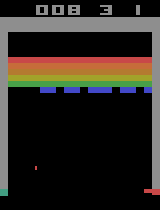
\includegraphics[width=\linewidth]{images/frame-sequence-2.png}
\end{subfigure}
\hfill
\begin{subfigure}[h]{0.19\linewidth}
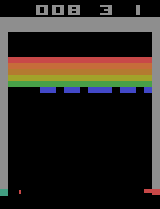
\includegraphics[width=\linewidth]{images/frame-sequence-3.png}
\end{subfigure}
\hfill
\begin{subfigure}[h]{0.19\linewidth}
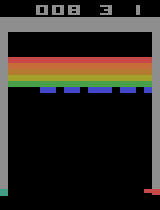
\includegraphics[width=\linewidth]{images/frame-sequence-4.png}
\end{subfigure}
\caption{Sequence of sampled frames}
\end{figure}

But we have found a trick to alleviate this problem. By default, Atari returns
an observation every 4 frames, and for each of those frames Atari performs the
same action we told it to execute. In practice a state-frame corresponds to 4
game-frame: at each state-frame the AI chooses an action that will be performed
for 4 game-frames, after which the environment will return a new observation,
that is a new state-frame. Increasing this number increases the number of times
the same action is performed, increasing the paddle movement from one
state-frame to another. This allows you to choose the same action for fewer
times in order to reach the opposite corner of the screen. That is, it
reduces N, thereby increasing the probability of this happening ($25\%^{N}$).
On the other hand, this makes it more difficult to hit the ball. Tests were
performed and optimal intermediate values were found for the frame skip,
between 10 and 14, which lead to a good increase in the score.

\subsubsection{The Non-Determinism Problem}

During the frame skip tests we noticed the problem that is the main difference between the two environments: non-determinism. When you perform an action in a state, it is not possible to know for sure what the next state will be like. This is not the case for PyGame. For Atari, this is because the amount of paddle movement is not fixed, but rather varies, partly randomly and partly according to the actions performed in previous states. It is even possible that, given a state and a movement action to be performed, the paddle will move into the next state in the opposite direction to that indicated, due to the inertia that the paddle has at that moment. In particular, without a frame skip, the paddle moves from -6 to +6 pixels. The skip of the frames, however, accentuates this problem, increasing the uncertainty of the movement from -6f to + 6f, with f the number of skipped frames from one state to another. To solve this problem at least partially, we inserted another variable in the state: move. It indicates the amount of movement performed with the last action, in order to have an estimate of the inertia of the paddle, and therefore know at least approximately where the paddle will go afterwards. The results of these tests are in point 1 of this section.

\subsubsection{The State Collision Problem}

The most serious problem, however, is the one introduced by non-determinism:
the collision of states, that is when two different states are represented in
the same way by the AI. The introduction of the variable move serves precisely
this, that is, to provide the algorithm of a sort of memory that indicates
more or less what the previous state was and, consequently, help to predict
the future state based on its own actions. However, this is not a definitive
solution. Suppose in fact that move indicates that the paddle has moved an
average amount between no movement (0) and maximum movement (6f). We do not
know if the paddle was accelerating or braking. We do not know if the previous
action was ``stand still'' and the paddle moved randomly by a lot, or if it was
``go right'' and the paddle randomly moved by a little bit. Suppose now that the
AI has learned that in a certain state, by performing a certain action, it
will get a reward. What happens now if, during the training phase, the AI
meets again the same state encountered some frames before, but in a different
circumstance? If the epsilon policy does not tell us to choose randomly,
we will obviously do the same action as before, but the result may not be the
same, we could lose the ball. Even worse is the case in which the epsilon
policy tells us to perform a random action, different from the optimal one,
but leads to a reward. In this case we are going to overwrite the information
of the optimal action on that state and moreover, since this reward is more
recent, it will have a higher value. So it will happen that, the next restart
of the game, when we meet the first occurrence of the double state, the AI
will perform the wrong action, losing not only the ball, but also all the
rewards we would have obtained following that path of actions leading to the
second occurrence of the state, the very same path that we had already explored
at the cost of so many clock cycles. Furthermore, the greater the distance
between the two occurrences of the conflicting state, the greater the loss of
rewards. This explains the fluctuating trend of the score during the training
phase, which is notably different from the PyGame case. So this is the main
reason for the difficulty of applying the Q-Learning or SARSA algorithms on
Atari Breakout.

\begin{figure}
\centering
\begin{subfigure}[h]{\linewidth}
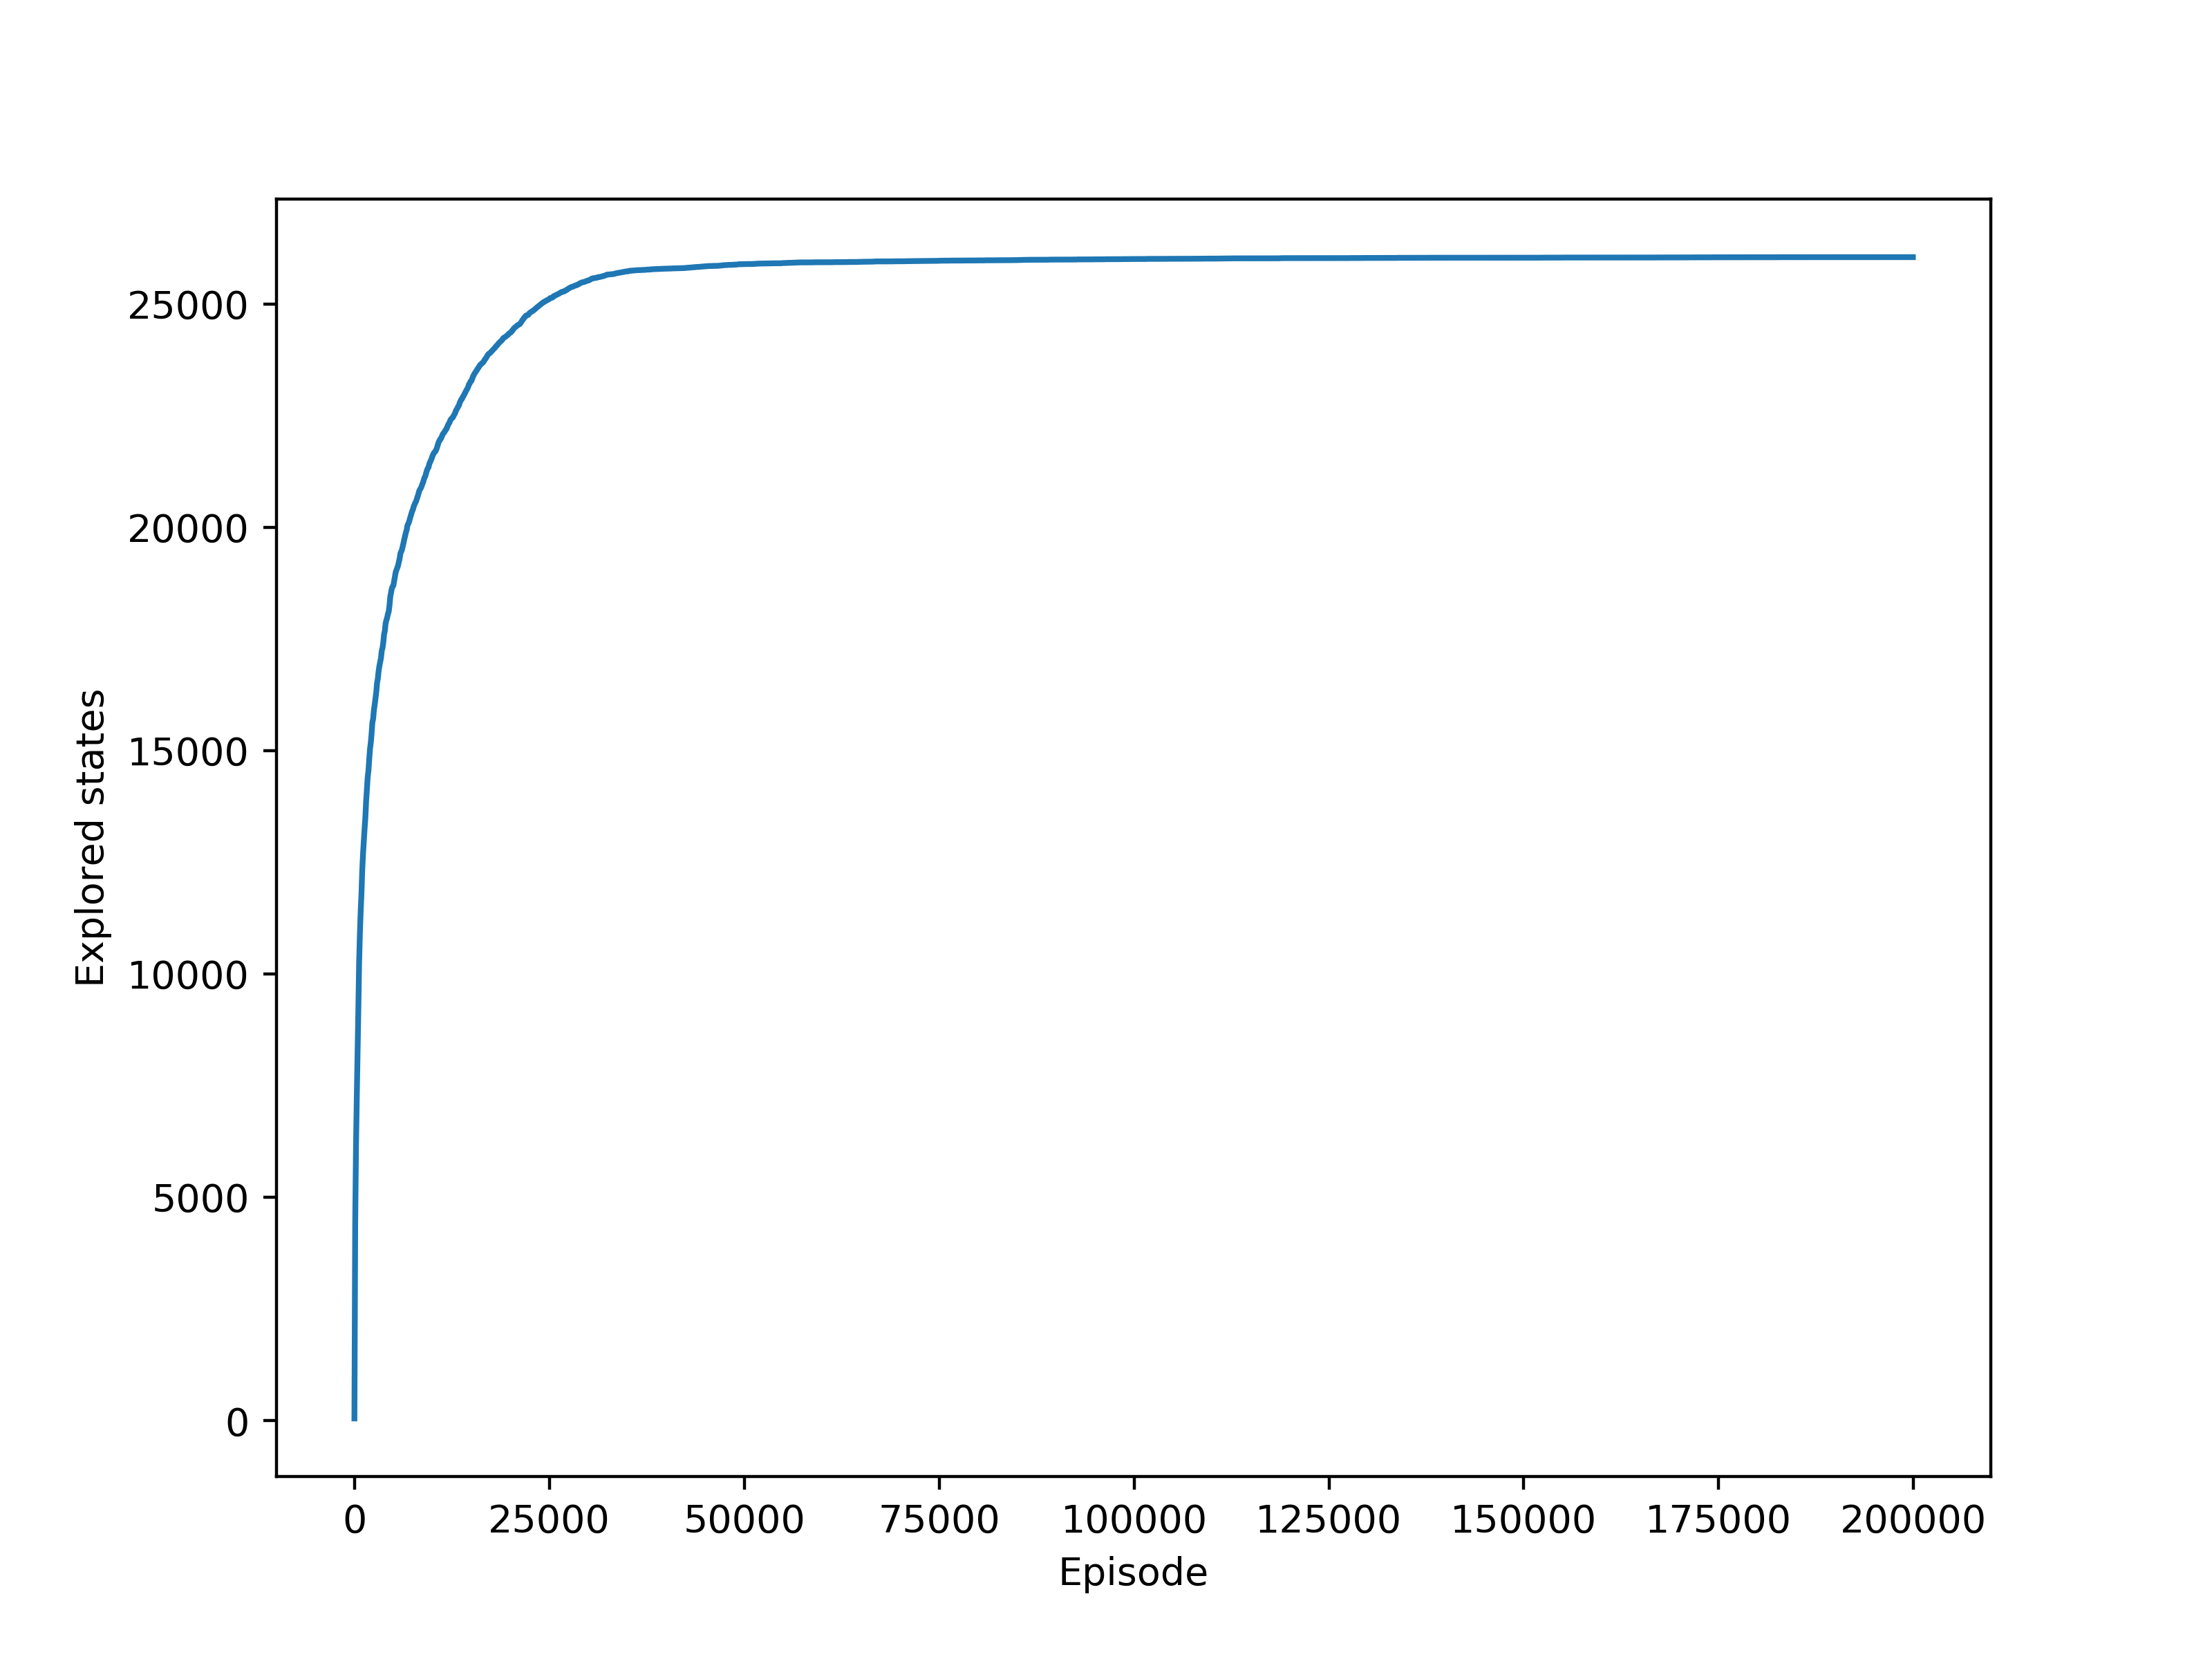
\includegraphics[width=\linewidth]{images/atari-ql-explored-states.png}
\centering
\end{subfigure}
\hfill
\begin{subfigure}[h]{\linewidth}
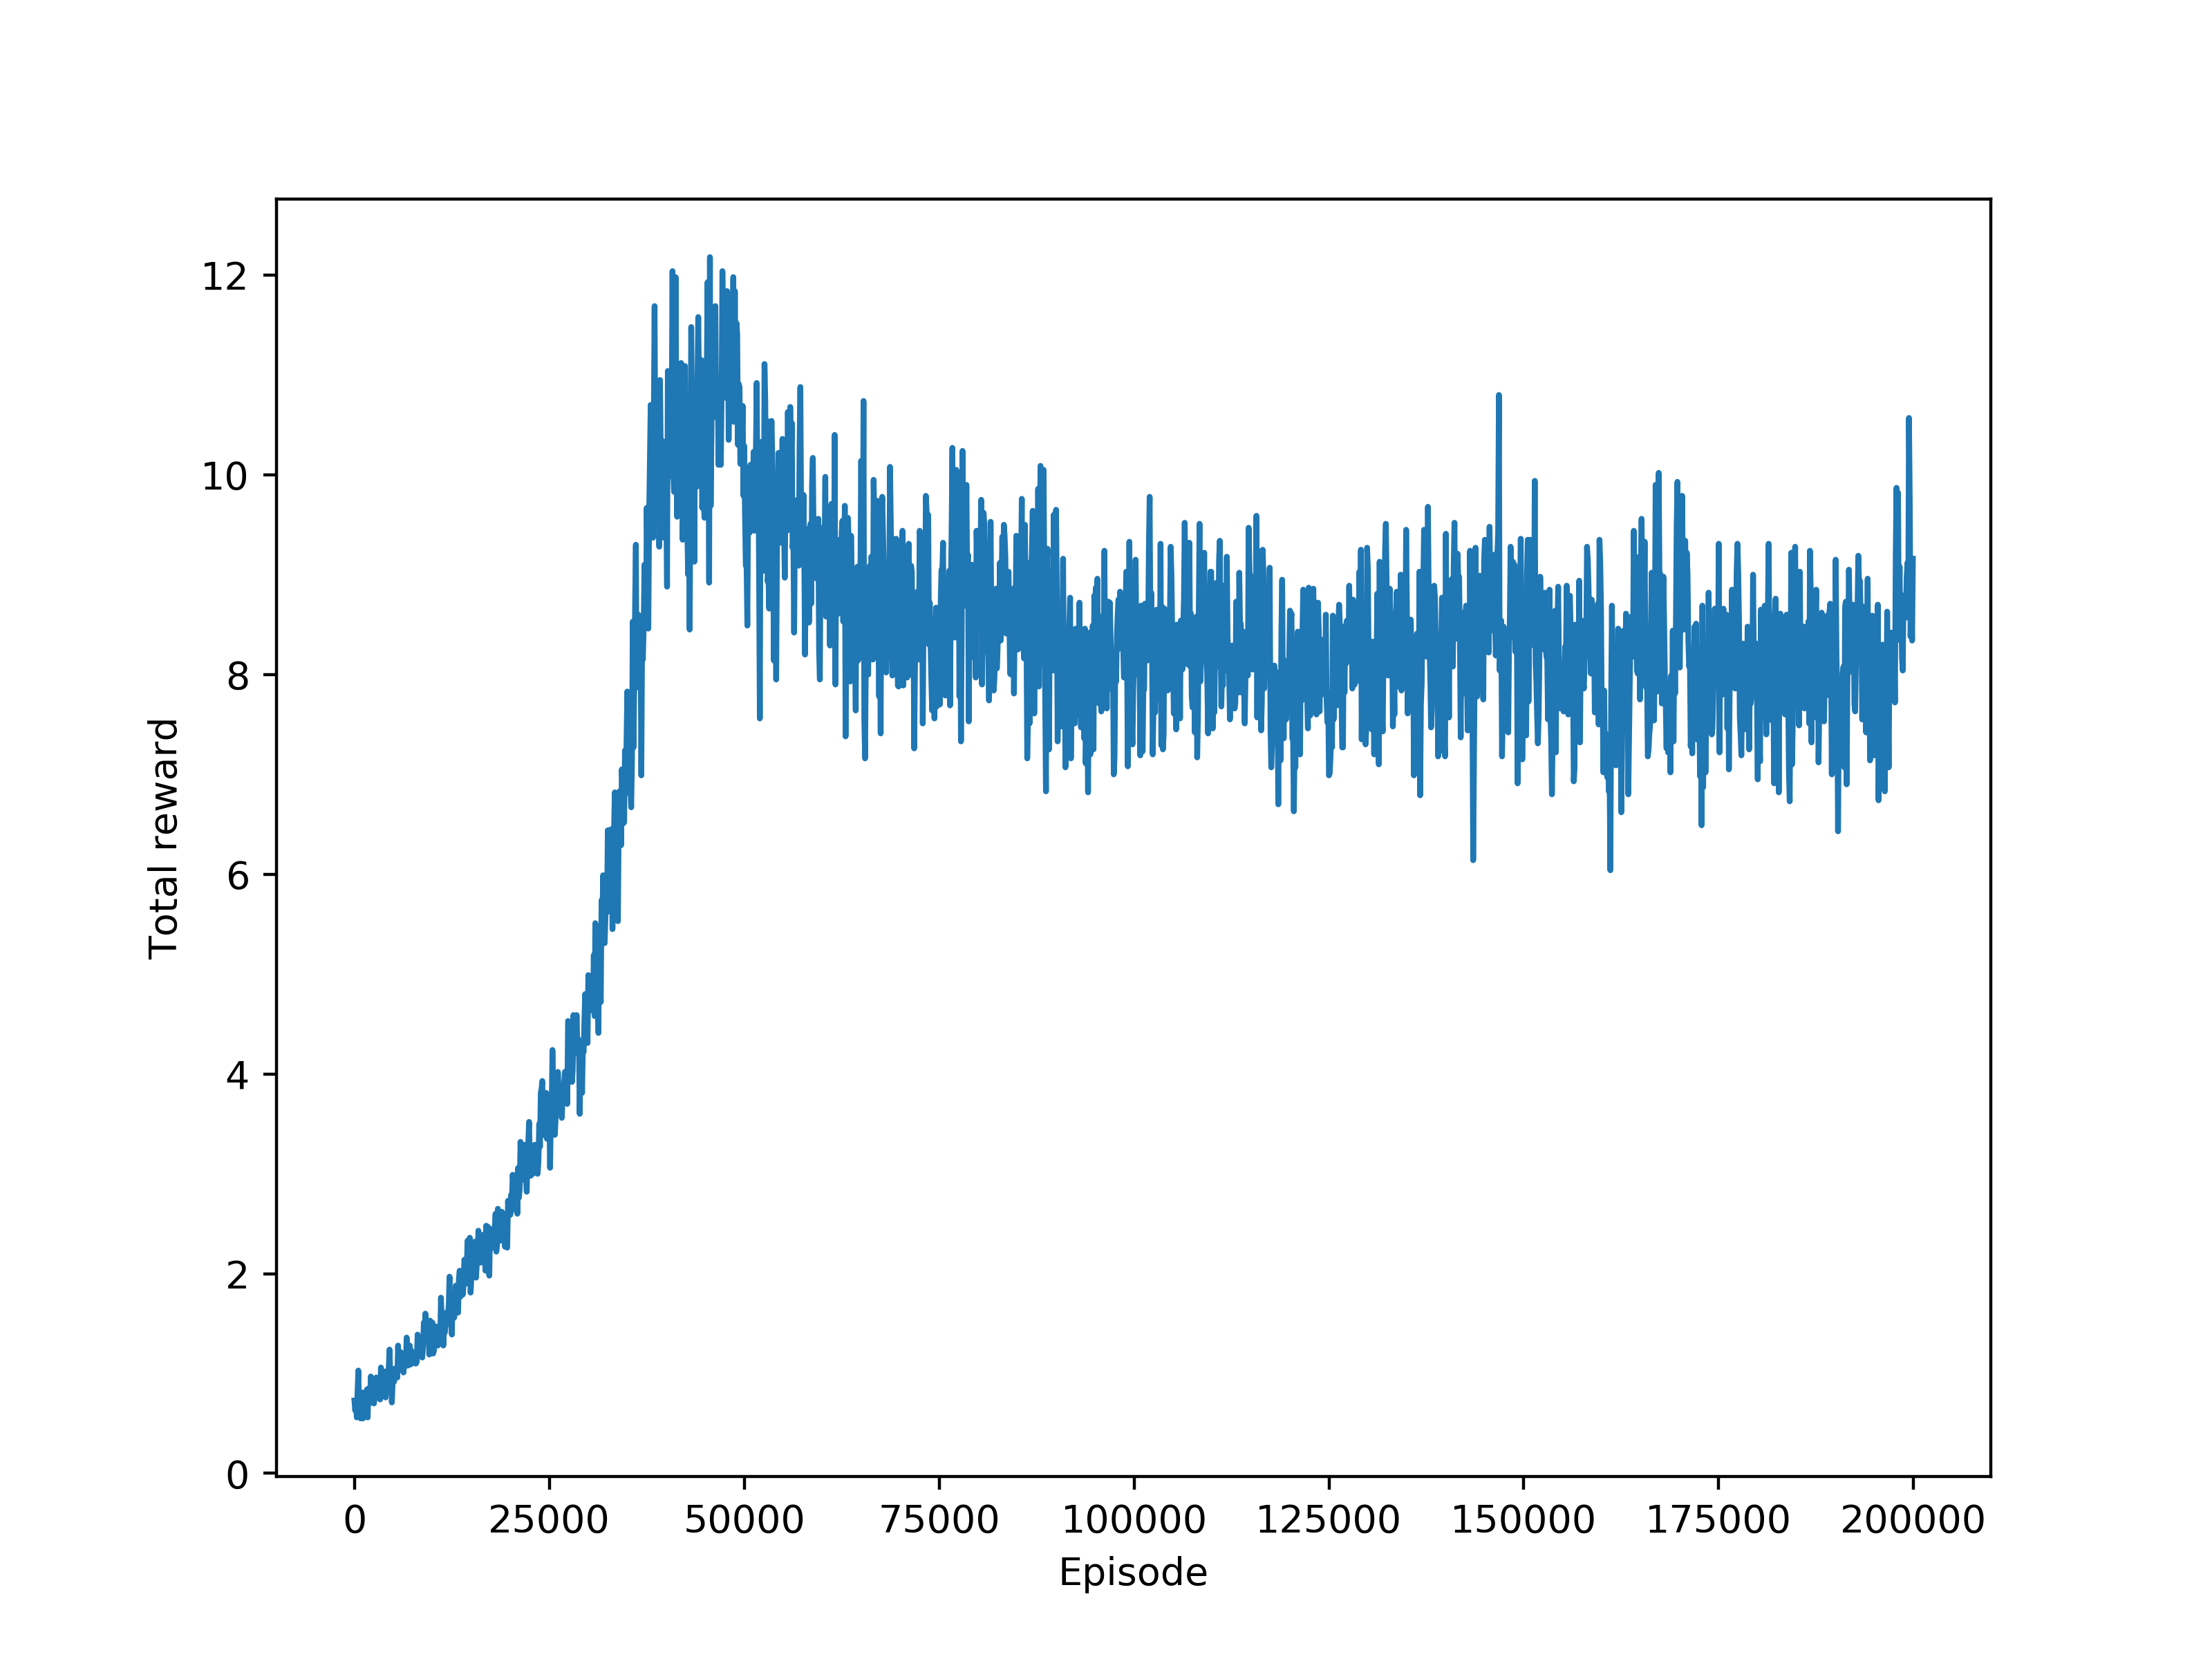
\includegraphics[width=\linewidth]{images/atari-ql-total-reward.png}
\centering
\end{subfigure}
\caption{Plots from the Atari Environment experiments. The reinforcement learning algorithm used in this experiment is Q-Learning.}
\end{figure}
